\\
The objective is to design a two level three phase inverter to drive the go karts PMSM motor. This basically consist of six switches and some capacitance on the DC-link. On figure \ref{fig:Sketch_PowerBoard} a simple model of the Power board is shown.

    \begin{figure}[H]
		\centering
		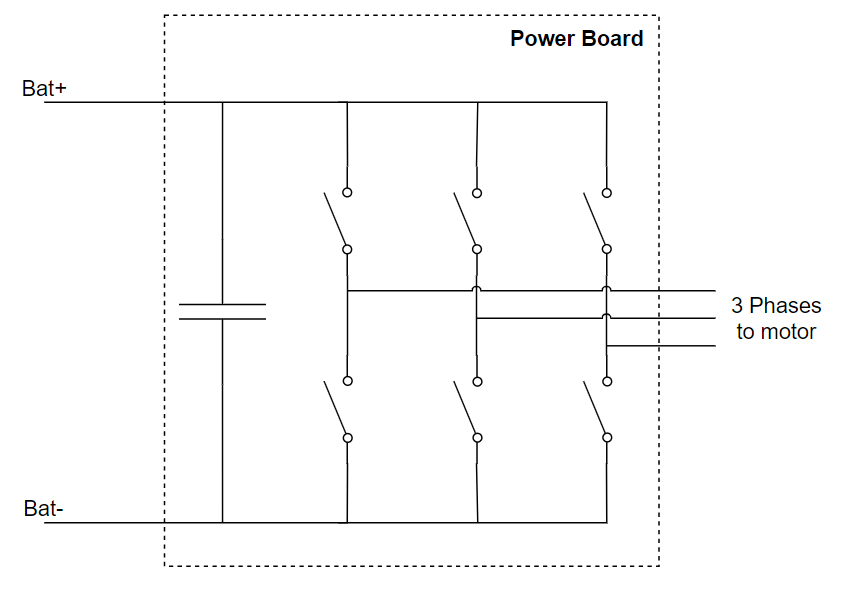
\includegraphics[width=0.7\textwidth]{pictures/hardware/Power_Board/Sketch_of_powerBoard.PNG}
		\caption{Sketch of the Power Board}
		\label{fig:Sketch_PowerBoard}
	\end{figure} 
	
This means that a switch component needs to be selected. The switch component has a great impact on the inverter design, due to the fact that it's main source of losses in the inverter. It is therefore important to choose a good transistor for switching. Besides the transistor choice, a good PCB layout and design is needed, because of heat transmission from the transistors.

\subsubsection{Switching frequency} \label{switching_frequency}
When deciding a switching frequency for the inverter, the rotation frequency of the motor is need to ensure, a high enough frequency. It is known from the motor parameters \ref{Motor_parameters_list}, that the maximum rotation speed  is $5000 rpm$ and it has 8 poles that equals to 4 pole pairs. From this the maximum frequency of the electrical field be determined.

\begin{equation}
    f = \frac{v_{rpm} \cdot P}{60}
    \label{eq:max_frequency}
\end{equation}

Where $v_{rpm}$ is the rotational speed in $rpm$ and $P$ is the number of pole pairs in the motor.
From equation \ref{eq:max_frequency} the maximum frequency of the electrical field is $333.3 Hz$.
It is desired to have between 10 and 20 switch periods per period of the electrical field. 20 switch periods per electrical field period results in a switching frequency of $6666 Hz$. It is not necessary to switch faster than the $6666 Hz$, but it's decided to use a switching frequency of $10 kHz$. This choice gives the possibility of having smaller capacitors, a higher frequency would decrease the switching loss, but didn't seen necessary. 
%This is done to make the use of smaller capacitors possible and because already so low frequency it is not a problem to increase it a bit. It is decided not to increase the switching frequency to more than $10 kHz$ to reducing the switching losses.


\subsubsection{PCB selection}   \label{PCB_selection}
Two types of PCB's has been considered, a ordinary multi-layer PCB and a single-layer aluminum PCB. There is of course pros and cons for both options. With the ordinary PCB there is better opportunities for conducting the heat away from the switch components. On the other hand it's not possible to use SMD components, due to the heat not being able to transfer away from the components. SMD components can result in a better and more compact layout. This is because SMD components are smaller and are available with multiple source legs, which minimize the common source for the switch components. The Use of SMD components will be possible with the aluminum PCB. Due to that the SMD components have a smaller area, and the heat has to transfer through the aluminum PCB, the cooling of the components is a harder task. With the aluminum PCB it is not possible to use through hole components, which can have some cons when it comes to the mounting of the large capacitors for the DC-link. 

The ordinary PCB has also the benefit, that is has multiple layers. This could make it easier to layout a good power board. On the other hand, due to the budget, it will not be possible to get a PCB with much more than 2 layers anyways, maybe 4 layers. It is of course better than the single layer on the aluminum PCB. It is possible to get the aluminum PCB with two layers, but it will result in a  too high thermal resistance and price.

Based on these considerations, an aluminum PCB has been choosen,
%it is chosen to use the aluminum PCB, 
because the benefits of the SMD components is weighted higher than the cons.


\subsubsection{Transistor selection}
Transistor selection is an important aspect in the design of the inverter. This is because that the transistors has great affect on the power loss in the system and thus the heat dissipation which set limitations on design. Transistor selection is made from a couple of factors. First of all the needed ratings necessary for the system. The Drain to Source current has to be minimum rated for $300 A$ if no parallel devices is used. It is chosen that the rated Drain to Source voltage should be around $100 V$. This is due to the battery in the go kart has a maximum voltage of $57.6V$, plus some safety margin for voltage spikes. The maximum battery voltage is found based on the cell voltage of a $LiFePO_4$: $3.6 V$, multiplied with the number of cells, which is 16. The transistor has to have a fall time of less than $250ns$ and rise time of less than $50ns$. The transistor also has to have the lowest possible on-resistance, to minimize conduction losses, which is very significance when conducting a current of $300A$.

The Transistor with these specifications and the lowest possible Drain-Source on resistance, to a affordable price, was a MOSFET. The MOSFET have the benefit of having a low current needed for turn on, the ability to handle high current needed for the motor and fast enough for the switching frequency. Since price is everything, when it comes to choice of components, then some sort of compromise will be made \\

The MOSFET chosen is an Infineon "IPB017N10N5". Some of the important specifications is listed in the table below.
\begin{table} [H]
\centering
 \begin{tabular}{|c|c|c|} 
 \hline
 \textbf{Parameters} & \textbf{Value} & \textbf{Unit} \\
 \hline
 \textbf{$V_{DS}$} & $100$ & $V$ \\  
 \hline
 \textbf{$R_{DS-ON}$} & $1.7$ & $m\Omega$ \\
 \hline
 \textbf{$I_D$} & $273$ & $A$ \\
 \hline
 \textbf{$Q_G\ (0-10V)$} & $168$ & $nC$ \\
 \hline
 \textbf{$Q_{GD}$} & $34$ & $nC$ \\
 \hline
 \textbf{$Q_{GS}$} & $53$ & $nC$ \\
 \hline
 \textbf{$Q_{sw}$} & $51$ & $nC$ \\
 \hline
 Rise time & $23$ & $ns$ \\
 \hline
 Fall time & $27$ & $ns$ \\
 \hline
\end{tabular}
\caption{Transistor parameters taken from the "IPB017N10N5" datasheet}
\end{table}

When looking at the parameters, a couple of things need to be considered. From the top it can be seen that the Drain-Source voltage is $100 V$, so it is able to handle the kart's battery voltage with safety. Next the [$I_D$] is not $300 A$ or above, which leads to a design choice of having two or more in parallel. Having more transistors in parallel has the benefit of splits the current up between them, lowering the conduction power loss. Having lower power loss decreases the amount of heat generated, which leads to less risk of overheating. The gate charge is the amount of charge that needs to be delivered to the transistor gate from the driver circuit, in order to turn the transistor on. This parameter needs to be as low as possible, same as the Drain-Source resistance, but normally with a low resistance comes higher gate charge and vise versa. In this case is it more important that the Drain-Source on resistance is low rather than the Gate charge is low. This is the case because speed of the turning on and off of the MOSFET is reduced anyway. Looking at the increased in driver power losses, the loss will not be as significant as the increase in power losses in a MOSFET with higher Drain-Source on resistance.\\ 


\subsubsection{Power and heat dissipation in the transistors}
There are two types of power losses in the transistors. One is conduction losses, which is caused by the intern resistance in MOSFET between the Drain and the Source, when the MOSFET is conducting. The other one is switching losses, which appears when the MOSFETs is turning on and off. Based on the power loss calculations the expected heat increase of the MOSFETs can be estimated, which will be used to decide, how many MOSFETs in parallel is needed.

\paragraph{Conduction power loss}
When a MOSFET is conducting there will be a power dissipation due to the internal Drain-Source on resistance in the MOSFET. Thus the conduction power loss in the MOSFETs is calculated in the same way as the power loss in a resistor. Equation \ref{eq:ConductionLossMOSFET} describes the conduction power loss for one MOSFET, $P_{con/MOSFET}$.

    \begin{equation}
        P_{con/MOSFET} = \bigg( \frac{I}{N \cdot 2} \bigg) ^2 \cdot R_{DS-ON}
        \label{eq:ConductionLossMOSFET}
    \end{equation}

$I$ is the peak current, $N$ is the number of transistors in parallel per switch, and $R_{DS-ON}$ is the Drain-Source on resistance of the MOSFET.
The peak current is divided by the number of transistors in parallel, to get the current in one MOSFET. Because the current is sinusoidal and the average duty cycle of the PWM over a period is $50 \% $, it is also divided by two to get the current one transistor is conducting.

To calculate the conduction power loss for all the transistors, it is then multiplied with the number of parallel MOSFETs per switch, two for taking both the high and low side into account, and the number of legs in the inverter, which is three.

    \begin{equation}
        P_{con} = \bigg( \frac{I}{N \cdot \sqrt{2}} \bigg) ^2 \cdot R_{DS-ON} \cdot N \cdot 2 \cdot 3
        \label{eq:ConductionLossTot}
    \end{equation}

On figure \ref{fig:ConductionLoss} the relationship between conduction power loss per MOSFET, equation \ref{eq:ConductionLossMOSFET}, and for all the MOSFETs, equation \ref{eq:ConductionLossTot}, is plotted as a function of the number of MOSFETs in parallel. 

    \begin{figure}[H]
		\centering
		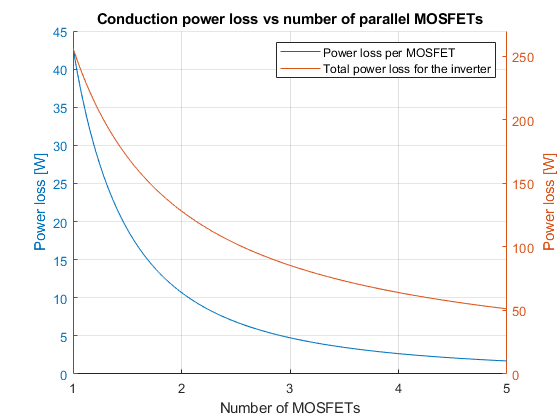
\includegraphics[width=0.8\textwidth]{pictures/hardware/Power_Board/Conduction_loss.png}
		\caption{Conduction power loss versus the number of parallel MOSFETs in parallel per switch. The blue curve describes the power loss per MOSFET and the red describes the total power loss}
		\label{fig:ConductionLoss}
	\end{figure} 

For figure \ref{fig:ConductionLoss} the peak current, $I$, is set to $300 A$, and the Drain-Source on resistance, $R_{DSon}$, is set to ${1.9 m \Omega}$, which is value at $80 \degree C$. \todo{ref to data sheet}

On figure \ref{fig:ConductionLoss} it can be seen that the more MOSFETs there are placed in parallel per switch, the conduction power losses reduces exponentially, for both each MOSFET and for the hole inverter.

\paragraph{Switching power loss}
The other cause of power loss in the MOSFETs is the switching power loss. The switching power losses is caused by the period, when switching, where both the voltage over and the current through the MOSFET is not zero. This is called hard switching. Soft switching is when the MOSFET switching on or off without the voltage and current overlaps. This will not cost any power loss. This is illustrated on figure \ref{fig:HardSoftSwitch}.

    \begin{figure}[H]
		\centering
		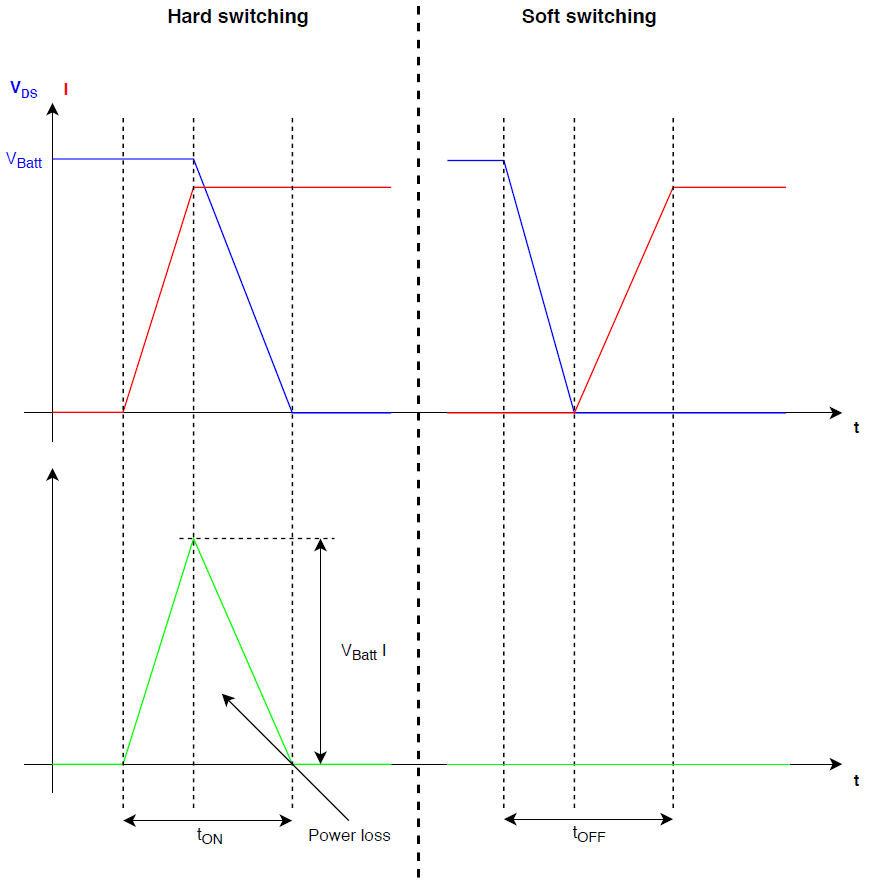
\includegraphics[width=0.8\textwidth]{pictures/hardware/Power_Board/Hard_soft_switching.PNG}
		\caption{Illustration of hard and soft switching of MOSFET}
		\label{fig:HardSoftSwitch}
	\end{figure} 

When running the motor, the motor current has a positive and a negative half cycle. During the positive half period the current going into the motor, and in the negative half period the current going from the motor into the inverter. In the positive half period the low-side switch gets soft turned on and the high-side switch gets hard turned on. Opposite in the negative half period the low-side switch is hard turned on and the high-side switch is soft turned on. This means One transistor will only hard switch $50 \%$ of the time.

The switching power is calculated as the area under the green line on figure \ref{fig:HardSoftSwitch} multiplied with the switching frequency. This is multiplied with a half because the switches is only hard switched $50 \%$ of the time, and therefore the Power loss is the half. 

    \begin{equation}
        P_{sw/MOSFET} = 0.5 \cdot 0.5 \cdot V_{batt} \cdot \frac{I}{N} \cdot (t_{on}+t_{off}) \cdot f_{s}
        \label{eq:sw_loss_MOSFET}
    \end{equation}

Where $V_{batt}$ is the battery voltage, $t_{on}$ is the turn on time, $t_{off}$ is the turn off time and $f_{s}$ is the switching frequency of the transistors.
Equation \ref{eq:sw_loss_MOSFET} is the switching power loss per MOSFET. To get the switching power loss for all of the MOSFETs in the inverter, this has to be multiplied with the number of parallel MOSFETs, two to take both the high- and low-side into to account, and the number of phases, which is three.

    \begin{equation}
        P_{sw} = 0.5 \cdot 0.5 \cdot V_{batt} \cdot \frac{I}{N} \cdot (t_{on}+t_{off}) \cdot f_{sw} \cdot N \cdot 2 \cdot 3
        \label{eq:sw_loss}
    \end{equation}
    
From this equation, a curve of the switching power loss in one MOSFET and in all the MOSFETs versus the number of the parallel MOSFETs, is made.

    \begin{figure}[H]
		\centering
		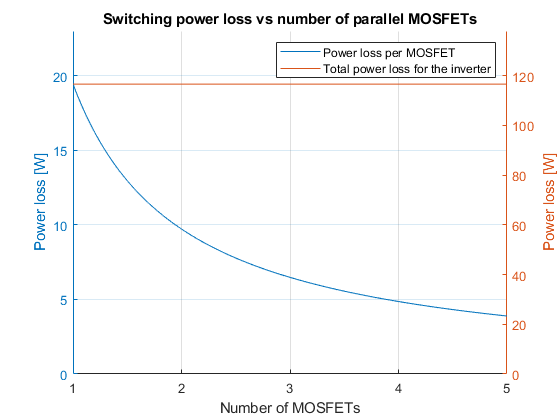
\includegraphics[width=0.8\textwidth]{pictures/hardware/Power_Board/Switch_loss.png}
		\caption{Switching power loss versus the number of parallel MOSFETs in parallel per switch. The blue curve describes power loss per MOSFET and the red describes the total power loss.}
		\label{fig:sw_loss}
	\end{figure}
	
Again is the peak current, $I$, is set to $300 A$. The battery voltage, $V_{batt}$, is set to $57.6 V$ and the switching frequency is set to the chosen frequency: $10 kHz$. The turn on time, $t_{on}$, and the turn off time, $t_{off}$, is calculated with the following equations.

    \begin{equation}
        t_{on} = \frac{Q_{sw}}{I_{GSource}}
    \end{equation}
    
    \begin{equation}
        t_{off} = \frac{Q_{sw}}{I_{GSink}}
    \end{equation}
    
Where $Q_{sw}$ is the switching charge of the MOSFET, which is stated in the Data sheet.\cite{mosfet}
$I_{GSource}$ and $I_{GSink}$ is respectively the current the driver deliverers to the Gate of the MOSFET when turning the MOSFET on and off. These are calculated in section \ref{sec:DriverDesign}. The turn on and off end up being $75 ns$ and $375 ns$, which could be faster, but is chosen to be limited to this. This is due to reducing high-frequency ringing when switching the MOSFETs. This results in a higher switching power loss, but because the switching loss does not have that big of an impact on the total power loss, due to the low switching frequency, it is not considered a problem.

On figure \ref{fig:sw_loss} it can be seen that the switching power loss of each MOSFET is reduced with number of parallel MOSFETs, but the over all power loss of the inverter is the same independent of the number of parallel MOSFETs.

\paragraph{Heat dissipation}
When the conduction power loss and switching power loss is determined compared to the number of MOSFETs, the total power losses is known. From the total power loss in the transistors, the heat dissipation can depending on the number of MOSFETs, be determined.

When determining the heat dissipation of the inverter, all the thermal resistances between the junction of the MOSFET and the ambient has to be specified.
First of all there is the internal junction to case resistance for the MOSFET.
When using the aluminum PCB with the SMD components, the heat has to be transferred through the PCB. This means this adds an extra thermal resistance to the system. The aluminum PCB is divided into three parts, the copper layer, a dielecrical layer for isolating the copper from the aluminum, and the aluminum layer.
Then there is a thin layer of thermal paste to connect the PCB to the heat sink. And the last resistance before the ambient is the heat sink. This is illustrated on figure \ref{fig:thermal_overview}.

    \begin{figure}[H]
		\centering
		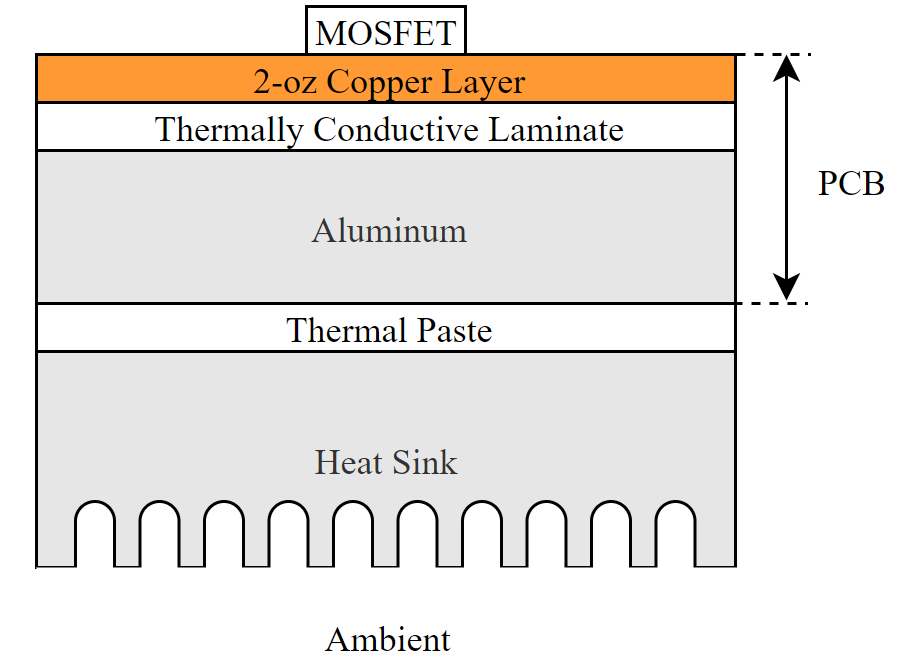
\includegraphics[width=0.6\textwidth]{pictures/hardware/Power_Board/Thermal_overview.png}
		\caption{Overview of the thermal resistances between the junction of the MOSFET and ambient}
		\label{fig:thermal_overview}
	\end{figure}
	
The thermal resistance from the junction to the case of the MOSFET is stated to be $0.4 K/W$ in the data sheet for the MOSFET.\cite{mosfet}
The thermal resistance of the copper layer, is calculated from equation \ref{Rthermal}

    \begin{equation}
        R_{thermal} = \frac{t_{layer}}{A_{MOSFET} \cdot k_{material}} 
        \label{Rthermal}
    \end{equation}
    
Where $t_{layer}$ is the thickness of the layer in $m$, $A_{MOSFET}$ is the surface area of the MOSFET in $m^2$, and $k_{material}$ is the thermal conduction constant for the layer material in $\frac{W}{m \cdot K}$.

The thickness of the copper layer is known to be $1 oz/foot^2$ from 'pcbway.com', which is converted to $34 \cdot 10^{-6} m$ from the density of copper. The surface area of the MOSFET is found in the data sheet to be $63 \cdot 10^{-6} m^2$.\cite{mosfet} The area of the MOSFET is used all the way down to the heat sink, because it is assumed that the heat will go straight through the PCB and the paste. This is most likely not the case but that will be the worst case.
The thermal conduction constant of copper is $401 \frac{W}{m \cdot K}$.\cite{toolbox}

The thermal resistance of the dielectrical layer is calculated based on the same equation as \ref{Rthermal}.

Where the thickness of the dielectrical layer is $100 \mu m$, which is stated by the manufactore, pcbway.com. The thermal conduction constant is chosen to be $1 \frac{W}{m \cdot K}$. The manufacture also offers the aluminum PCB with a dielectrical layer with a thermal conduction constant of $2 \frac{W}{m \cdot K}$, but due to price this was not chosen.

Equation \ref{Rthermal} is used again for calculating the thermal resistance of the aluminum layer of the PCB.
Where the he thickness of the aluminum layer is the chosen PCB thickness of $0.8 mm$ minus the thickness of the two other layers. The thickness of $0.8 mm$ is chosen because that is the thinnest option without getting the PCB to increase in price. The thermal conduction constant for aluminum is $236 \frac{W}{m \cdot K}$.\cite{toolbox}

The thermal resistance for the total PCB is then:

    \begin{equation}
        R_{PCB} = R_{copper} + R_{del} + R_{alu}
        \label{RPCB}
    \end{equation}

Where $R_{copper}$ is the thermal resistance of the copper layer, $R_{del}$ is the thermal resistance of the dielectrical layer, and $R_{alu}$ is the thermal resistance of the aluminum layer.

To calculate the thermal resistance of the thermal paste, equation \ref{Rthermal} is used as well. The thickness of the paste is estimated to be $0.1 mm$ and the thermal conduction constant of the paste is set to $3 \frac{W}{m \cdot K}$. This based on values for different thermal paste, and then a value close to the average of them was chosen.

This results in, that the total temperature difference from the thermal paste to the MOSFET junction can be calculated with equation \ref{eq:tempMOSFET}.

    \begin{equation}
        T_{JP} = P_{loss/MOSFET} \cdot (R_{JC} + R_{PCB})
        \label{eq:tempMOSFET}
    \end{equation}
    
Where $R_{JC}$ is the internal junction to case thermal resistance and $P_{loss}$ is the total power loss for one MOSFET. 

To calculate the temperature difference over the heat sink, the average power loss is used instead of the maximum power loss. This is done because the heat sink has a higher thermal capacitance, and therefore is less reactive to changes in temperature. The average power loss is calculated in the same way as the maximum power loss, but instead of using the maximum current a average current is estimated. The average current is estimated to $75 A$.
From this the temperature difference over the heat sink is calculated, with equation \ref{Theatsink} 

    \begin{equation}
        T_{HA} = P_{Avg} \cdot R_{HA}
        \label{Theatsink}
    \end{equation}

The $P_{Avg}$ is the average power loss for all the MOSFETs and $R_{HA}$ is the thermal resistance of the heat sink. 

The final temperature difference from ambient to the junction of one MOSFET is then:

    \begin{equation}
        T_{J} = T_A + T_{HA} + T_{JP}
        \label{Theatsink}
    \end{equation}
    
Where the $T_A$ is the ambient temperature. It has to be notices that the temperature difference over the heat sink is depending on the total power loss, and the temperature difference from the paste to the junction of a MOSFET is depending on the power loss for one MOSFET. This is due to that the thermal resistance of the heat sink is common for all MOSFETs and there is a parallel thermal resistance for each MOSFET from the paste to the junction.

On figure \ref{fig:junctionTemp} is the relationship between the junction temperature of the MOSFETs and the number of MOSFETs in parallel showed. 

    \begin{figure}[H]
		\centering
		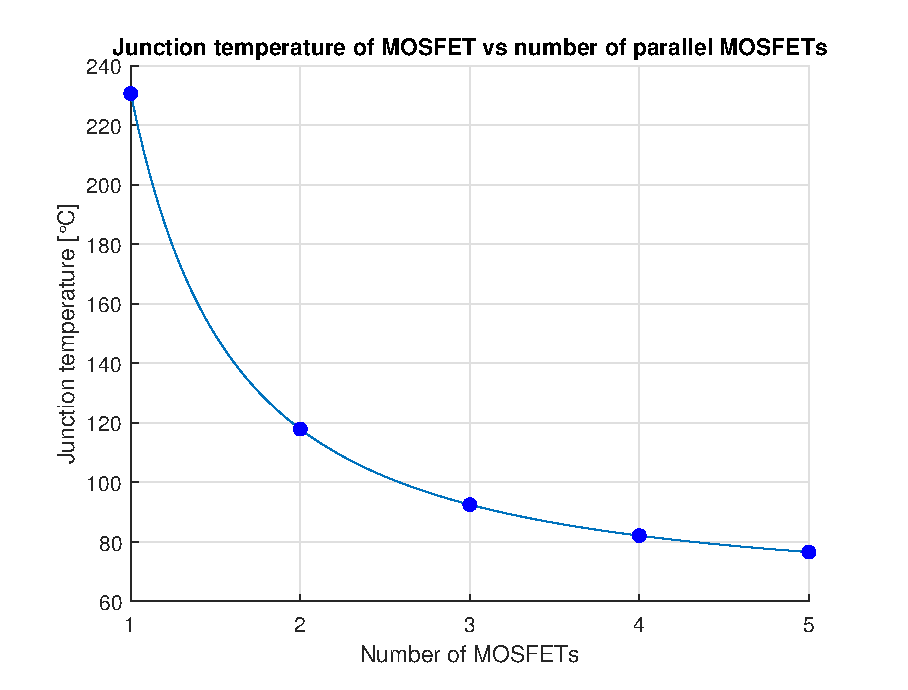
\includegraphics[width=0.8\textwidth]{pictures/hardware/Power_Board/Juntion_temp.eps}
		\caption{Junction temperature versus the number of transistors in parallel per switch}
		\label{fig:junctionTemp}
	\end{figure}

Based on figure \ref{fig:junctionTemp} it is decided to use two MOSFETs in parallel per switch. Because the Power board only got one layer, it is preferred to have as few MOSFETs as possible, to avoid making the layout of the Power board to complicated. From figure \ref{fig:junctionTemp} it can be seen that the junction temperature of the MOSFETs are going to be $118 \degree C$. This is a bit high temperature, but considering that this will be the worst case, this is acceptable.